\documentclass[10pt, a4paper,english,spanish]{article}
%\documentclass[10pt,a4paper]{article}
\usepackage[utf8]{inputenc} % para poder usar tildes en archivos UTF-8
\usepackage[spanish]{babel} % para que comandos como \today den el resultado en castellano
\usepackage{caratula}
\usepackage{fullpage} %small margins
\usepackage[parfill]{parskip} %genera saltos entre parrafos
\usepackage[justification=centering]{caption}
\usepackage[usenames,dvipsnames,svgnames,table]{xcolor}
\usepackage{colortbl}
\usepackage[colorlinks=true, linkcolor=black]{hyperref} %Links + Links en el índice
\definecolor{gray}{gray}{0.35}
\definecolor{brightgreen}{rgb}{0.4, 1.0, 0.0}
\definecolor{ReallyLightGrey}{gray}{0.93}
\usepackage{listings}
\usepackage{enumitem}
\usepackage{amsmath} %big brackets
\usepackage[pdftex]{graphicx}
\usepackage[bottom]{footmisc}
\lstset{
    numbers=left,
    breaklines=true,
    tabsize=2,
    basicstyle=\ttfamily\color{gray},
}
\setlength{\parindent}{8pt}
\usepackage{mathtools}
\usepackage[margin=50pt]{geometry}
\usepackage{amsfonts}
\usepackage{flafter}
\usepackage{float}
\usepackage{pdflscape}
\restylefloat{table}
\setcounter{tocdepth}{5}
\setcounter{secnumdepth}{5}

\begin{document}

\materia{Seguridad de la Información}
\submateria{Primer Cuatrimestre de 2017}
\titulo{Trabajo Práctico}
\subtitulo{}

\integrante{Federico De Rocco}{403/13}{fede.183@hotmail.com}
\integrante{Francisco Muchinik}{238/14}{jmmassigoge@gmail.com}
\integrante{Yamil Alis}{742/00}{yamil.alis@gmail.com}
\maketitle
\newpage

\tableofcontents

\section{Servidor Syslog}
\subsection{Servidor syslog con forward integrity}
Para nuestro servidor syslog utilizamos \hyperlink{https://gist.github.com/marcelom/4218010 }{https://gist.github.com/marcelom/4218010} y, sobre este, implementamos nuestro 
mecanismo de logging seguro. Nos basamos en el paper [2] para construir nuestra solución. A continuación, describiremos nuestra implementación.
Generamos un MAC para cada log que no pueda ser modificado sin quedar en evidencia
aunque el sistema que genera los logs sea comprometido. La idea es que el sistema no repita la clave utilizada en los pasos anteriores. Una vez calculado
el MAC se debe descartar dicha clave para evitar que se la pueda obtener. Este proceso se muestra en la siguiente imagen:
\begin{figure}[H]
\centering
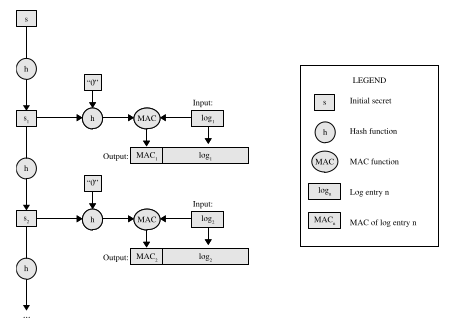
\includegraphics[scale=1]{imagenes/MAC.png}
\end{figure}
Para asegurar la propiedad descripta, generamos la clave actual en base a la inmediatamente anterior como se explica en [1].
Tenemos para el log número i la clave $K_{i}$ que se obtiene aplicándole una función no reversible a
$K_{i-1}$. Una vez calculada $K_{i}$, se borra $K_{i-1}$. Esto último requiere que el FI sea rápido. Si el atacante obtiene control del sistema en el momento que el siguiente log es el número i,
obtendría la clave $K_{i}$. Con la cual no puede regenerar $K_{i-1}$ ni ninguna de las anteriores.
A la hora de verificar el estado de un registro en particular calculamos su clave en la cadena de hash.
Al log guardado le aplicamos la función de hash con la que obtenemos el MAC. Si este no coincide con el almacenado,
el registro fue modificado. La siguiente imagen corresponde al proceso de verificación:
\begin{figure}[H]
\centering
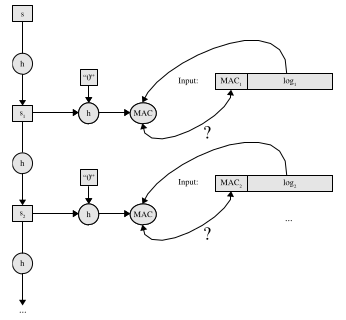
\includegraphics[scale=1]{imagenes/Verification.png}
\end{figure}
Omitimos la posibilidad de utilizar cifrado en los logs.
Nuestra implementación tiene las siguientes particularidades:
\begin{itemize}
\item Utilizamos un secreto inicial, elegido por el administrador del equipo, para iniciar el servidor syslog.
Para cada log que se genere, se calcula su MAC y se guarda.
\item El propio administrador realizara la verificación de los logs aportando el secreto inicial.
\item Los registros de eventos se guardan en un ".log" de solo lectura para un usuario normal.
\item Cada verificación realiza el procedimiento descripto para todos los logs en el registro.
\end{itemize}
\subsection{Alternativas de diseño: Verificación acumulativa}
En lugar de guardar un MAC por cada registro del log, alternativamente se puede guardar solamente uno resultante de un calculo acumulativo. Este mecanismo consiste en que la función de hash toma no solamente la clave, sino también el MAC calculado anteriormente. 
Utilizando esto podemos guardar en un lado el registro de logs y, en otro, el último hash de la cadena. 
Existe un problema en la verificación acumulativa dado que necesita todos los logs previos para comprobar uno. Suponiendo que un atacante modifique el log borrando una parte de él, dejando registros previos y posteriores a la modificación intactos. Tanto el método de verificación que nosotros usamos como su versión acumulativa, podrán detectar el cambio. Además, los dos serán capaces de verificar que los logs previos al ataque están correctos y se puede confiar en ellos. Sin embargo, la verificación acumulativa es incapaz de saber si los registros posteriores están correctos.   
\subsection{Alternativas de diseño: Clave pública}
Una alternativa al uso de la cadena de hash consiste en firmar los logs utilizando una clave privada y verificar la firma con su clave pública. La principal ventaja de esta implementación es que permite que la verificación se pueda realizar con una clave diferente de la que se usa para firmar. 
El proceso consiste en generar un par de claves de los cuales se debe guardar de forma segura la publica(debe asegurar integridad). Utilizando la clave privada se firma una entrada del log que consiste en una secuencia de $n$ claves publicas utilizadas para verificar los $n-1$ siguientes logs. La última clave publica de la secuencia se utilizara para verificar la siguiente entrada que contendrá otra secuencia de claves publicas y así sucesivamente. Cada clave privada usada en la secuencia se descarta inmediatamente. El objetivo es tener las claves publicas a mano para la verificación y, dado que se están firmadas, se puede corroborar su autenticidad. En las siguientes imágenes se muestra el proceso de logging seguro.
\begin{figure}[H]
\centering
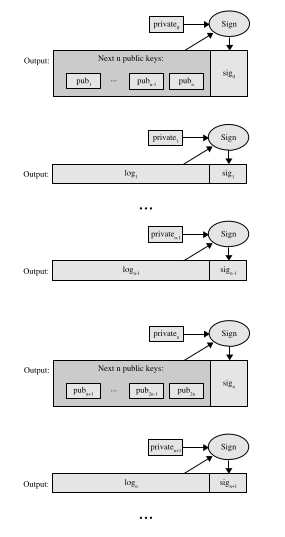
\includegraphics[scale=0.4]{imagenes/PublicKey.png}
\end{figure}
A la hora de verificar, se utilizara la clave publica inicial para el primer log que contiene la cadena de claves publicas. Si es correcto se verificaran cada uno de los siguientes $n$ logs utilizando esta secuencia. Se realizara el proceso para la siguiente entrada utilizando la ultima clave de la cadena y con esto se comprueba la siguiente cadena de claves publicas a utilizar para la verificación. La siguiente imagen ilustra el proceso.
\begin{figure}[H]
\centering
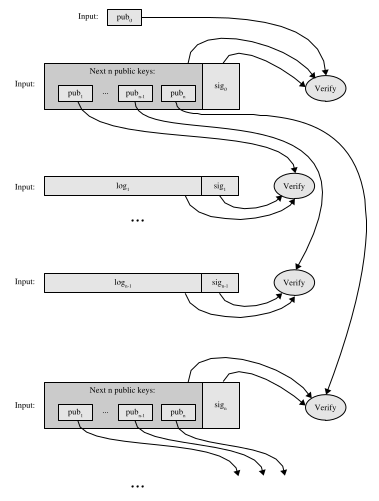
\includegraphics[scale=0.4]{imagenes/PublicKeyVerification.png}
\end{figure}
  
Además de la firma de los logs, se pueden utilizar las claves privadas para cifrar los logs, ocultando la información que contienen.

\section{Bibliografía}
\subsection{Bibliografía}



\begin{thebibliography}{9}
\bibitem{bio1} 
Logcrypt: Forward Security and Public Verification for Secure Audit Logs de Jason E. Holt.
\bibitem{bio2} 
Forward Integrity For Secure Audit Logs de Mihir Bellare y Bennet S. Yee.
\bibitem{bio3} 
Wikipedia. Merkle Tree.
\bibitem{bio4} 
Certificate Transparency RFC 6962.
\bibitem{bio5} 
Mastering Bitcoin. Andreas M. Antonopoulos. Cap\'itulo 7.
\bibitem{bio6} 
$https://gist.github.com/marcelom/4218010$

\end{thebibliography}

\end{document}
